	% !TeX spellcheck = en_GB
	\begin{figure}[!htb]
	  \setlength{\unitlength}{\textwidth}
	
	        \begin{picture}(1,0.75)(-0.02,-0.02)
	
	 
	      
	      \put(0.08,0.03){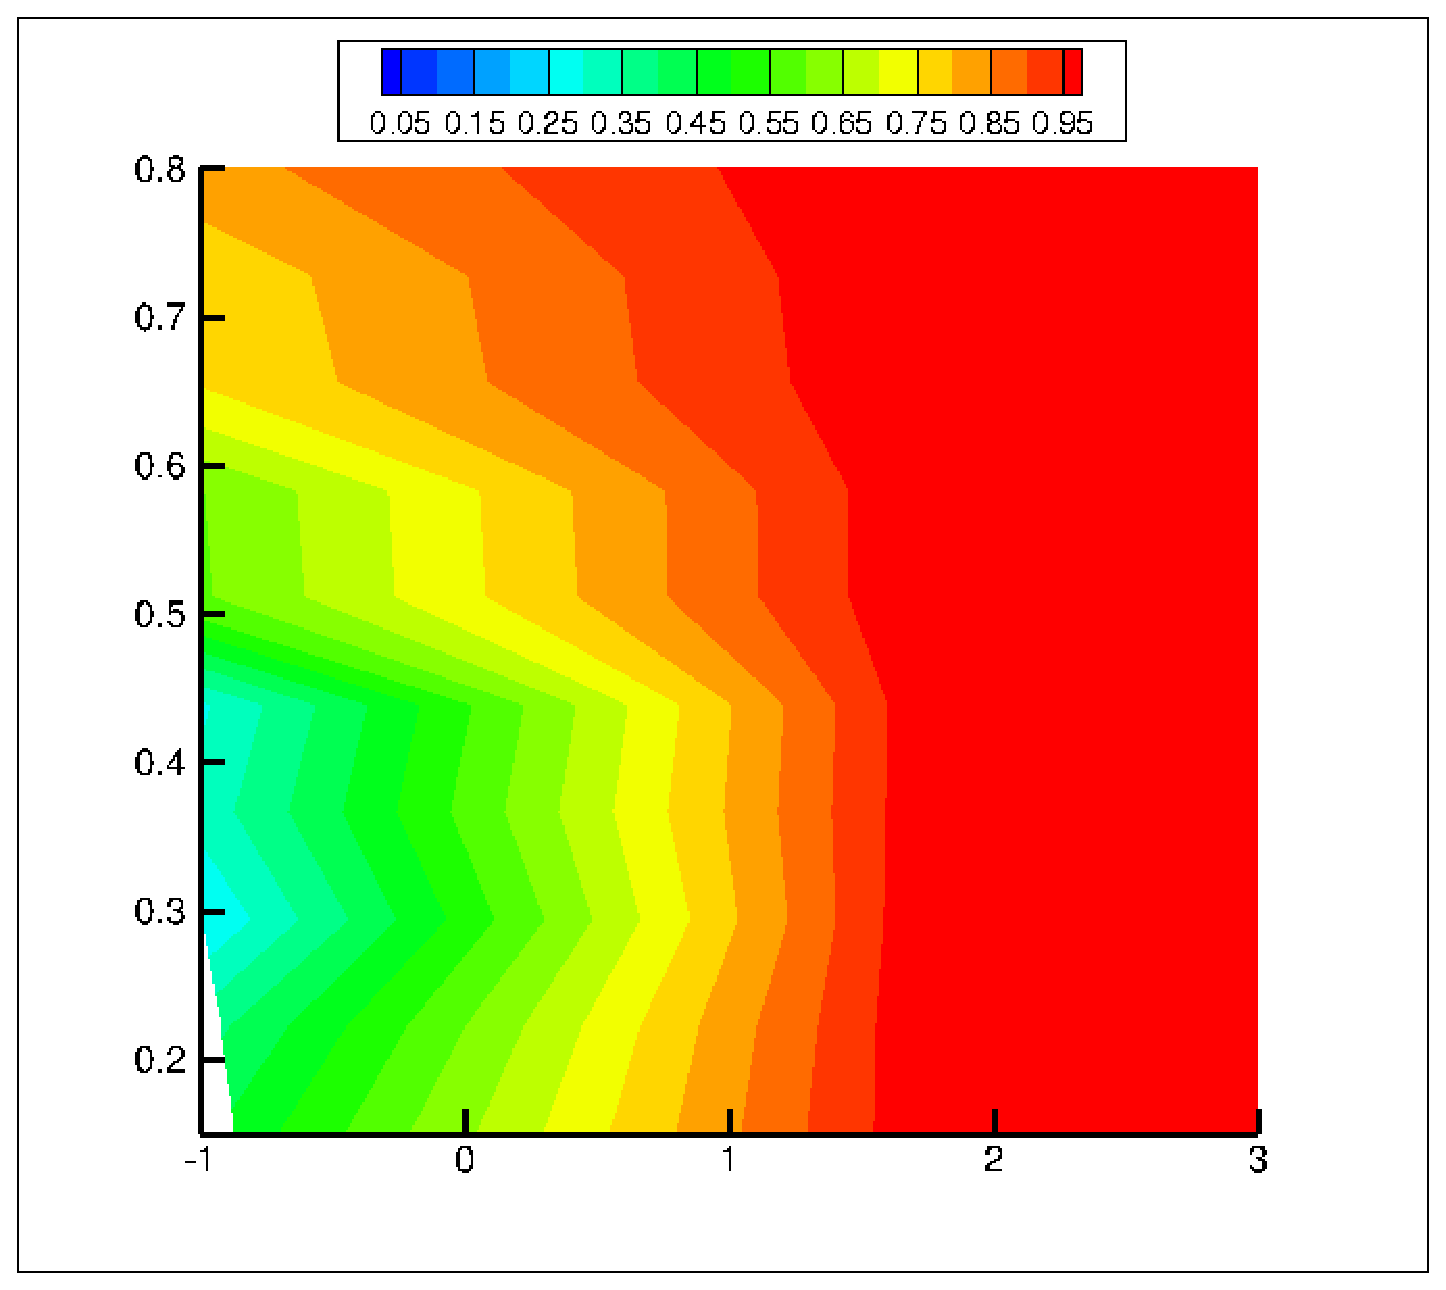
\includegraphics[width=0.75\unitlength]{./chapter-frequnecy-response/fnp/flin-fqss.eps}}
	
	      \put(0.1,0.33){\massdamp}
	      \put(0.45,0.06){$\massstiff$}
	      \put(0.18,0.65){$\frac{f_{lin}}{f_{QSS}}$}
	      
	      
	     
	       
	      
	
	      %\put(0.095,0.218){\small(a)}
	      %\put(0.565,0.218){\small(b)}
	      
	    \end{picture}
	
	  \caption{Contour plot of  $\frac{f_{lin}}{f_{QSS}}$ in \massstiff\ \massdamp\ space. The linear frequency \freqlin\ provides a good agreement with the frequency predicted by the quasi-steady state model beyond $\massstiff=10$}
	    \label{fig:freq-qss-linear}
	\end{figure}
	
	 %vspace{10cm}
